%% bare_jrnl.tex
%% V1.4b
%% 2015/08/26
%% by Michael Shell
%% see http://www.michaelshell.org/
%% for current contact information.
%%
%% This is a skeleton file demonstrating the use of IEEEtran.cls
%% (requires IEEEtran.cls version 1.8b or later) with an IEEE
%% journal paper.
%%
%% Support sites:
%% http://www.michaelshell.org/tex/ieeetran/
%% http://www.ctan.org/pkg/ieeetran
%% and
%% http://www.ieee.org/

%%*************************************************************************
%% Legal Notice:
%% This code is offered as-is without any warranty either expressed or
%% implied; without even the implied warranty of MERCHANTABILITY or
%% FITNESS FOR A PARTICULAR PURPOSE! 
%% User assumes all risk.
%% In no event shall the IEEE or any contributor to this code be liable for
%% any damages or losses, including, but not limited to, incidental,
%% consequential, or any other damages, resulting from the use or misuse
%% of any information contained here.
%%
%% All comments are the opinions of their respective authors and are not
%% necessarily endorsed by the IEEE.
%%
%% This work is distributed under the LaTeX Project Public License (LPPL)
%% ( http://www.latex-project.org/ ) version 1.3, and may be freely used,
%% distributed and modified. A copy of the LPPL, version 1.3, is included
%% in the base LaTeX documentation of all distributions of LaTeX released
%% 2003/12/01 or later.
%% Retain all contribution notices and credits.
%% ** Modified files should be clearly indicated as such, including  **
%% ** renaming them and changing author support contact information. **
%%*************************************************************************


% *** Authors should verify (and, if needed, correct) their LaTeX system  ***
% *** with the testflow diagnostic prior to trusting their LaTeX platform ***
% *** with production work. The IEEE's font choices and paper sizes can   ***
% *** trigger bugs that do not appear when using other class files.       ***                          ***
% The testflow support page is at:
% http://www.michaelshell.org/tex/testflow/



\documentclass[journal]{IEEEtran}
\usepackage{tikz}
%
% If IEEEtran.cls has not been installed into the LaTeX system files,
% manually specify the path to it like:
% \documentclass[journal]{../sty/IEEEtran}





% Some very useful LaTeX packages include:
% (uncomment the ones you want to load)


% *** MISC UTILITY PACKAGES ***
%
%\usepackage{ifpdf}
% Heiko Oberdiek's ifpdf.sty is very useful if you need conditional
% compilation based on whether the output is pdf or dvi.
% usage:
% \ifpdf
%   % pdf code
% \else
%   % dvi code
% \fi
% The latest version of ifpdf.sty can be obtained from:
% http://www.ctan.org/pkg/ifpdf
% Also, note that IEEEtran.cls V1.7 and later provides a builtin
% \ifCLASSINFOpdf conditional that works the same way.
% When switching from latex to pdflatex and vice-versa, the compiler may
% have to be run twice to clear warning/error messages.






% *** CITATION PACKAGES ***
%
%\usepackage{cite}
% cite.sty was written by Donald Arseneau
% V1.6 and later of IEEEtran pre-defines the format of the cite.sty package
% \cite{} output to follow that of the IEEE. Loading the cite package will
% result in citation numbers being automatically sorted and properly
% "compressed/ranged". e.g., [1], [9], [2], [7], [5], [6] without using
% cite.sty will become [1], [2], [5]--[7], [9] using cite.sty. cite.sty's
% \cite will automatically add leading space, if needed. Use cite.sty's
% noadjust option (cite.sty V3.8 and later) if you want to turn this off
% such as if a citation ever needs to be enclosed in parenthesis.
% cite.sty is already installed on most LaTeX systems. Be sure and use
% version 5.0 (2009-03-20) and later if using hyperref.sty.
% The latest version can be obtained at:
% http://www.ctan.org/pkg/cite
% The documentation is contained in the cite.sty file itself.






% *** GRAPHICS RELATED PACKAGES ***
%
%\ifCLASSINFOpdf
  % \usepackage[pdftex]{graphicx}
  % declare the path(s) where your graphic files are
  % \graphicspath{{../pdf/}{../jpeg/}}
  % and their extensions so you won't have to specify these with
  % every instance of \includegraphics
  % \DeclareGraphicsExtensions{.pdf,.jpeg,.png}
%\else
  % or other class option (dvipsone, dvipdf, if not using dvips). graphicx
  % will default to the driver specified in the system graphics.cfg if no
  % driver is specified.
  % \usepackage[dvips]{graphicx}
  % declare the path(s) where your graphic files are
  % \graphicspath{{../eps/}}
  % and their extensions so you won't have to specify these with
  % every instance of \includegraphics
  % \DeclareGraphicsExtensions{.eps}
%\fi
% graphicx was written by David Carlisle and Sebastian Rahtz. It is
% required if you want graphics, photos, etc. graphicx.sty is already
% installed on most LaTeX systems. The latest version and documentation
% can be obtained at: 
% http://www.ctan.org/pkg/graphicx
% Another good source of documentation is "Using Imported Graphics in
% LaTeX2e" by Keith Reckdahl which can be found at:
% http://www.ctan.org/pkg/epslatex
%
% latex, and pdflatex in dvi mode, support graphics in encapsulated
% postscript (.eps) format. pdflatex in pdf mode supports graphics
% in .pdf, .jpeg, .png and .mps (metapost) formats. Users should ensure
% that all non-photo figures use a vector format (.eps, .pdf, .mps) and
% not a bitmapped formats (.jpeg, .png). The IEEE frowns on bitmapped formats
% which can result in "jaggedy"/blurry rendering of lines and letters as
% well as large increases in file sizes.
%
% You can find documentation about the pdfTeX application at:
% http://www.tug.org/applications/pdftex





% *** MATH PACKAGES ***
%
\usepackage{amsmath}
% A popular package from the American Mathematical Society that provides
% many useful and powerful commands for dealing with mathematics.
%
% Note that the amsmath package sets \interdisplaylinepenalty to 10000
% thus preventing page breaks from occurring within multiline equations. Use:
\interdisplaylinepenalty=2500
% after loading amsmath to restore such page breaks as IEEEtran.cls normally
% does. amsmath.sty is already installed on most LaTeX systems. The latest
% version and documentation can be obtained at:
% http://www.ctan.org/pkg/amsmath





% *** SPECIALIZED LIST PACKAGES ***
%
%\usepackage{algorithmic}
% algorithmic.sty was written by Peter Williams and Rogerio Brito.
% This package provides an algorithmic environment fo describing algorithms.
% You can use the algorithmic environment in-text or within a figure
% environment to provide for a floating algorithm. Do NOT use the algorithm
% floating environment provided by algorithm.sty (by the same authors) or
% algorithm2e.sty (by Christophe Fiorio) as the IEEE does not use dedicated
% algorithm float types and packages that provide these will not provide
% correct IEEE style captions. The latest version and documentation of
% algorithmic.sty can be obtained at:
% http://www.ctan.org/pkg/algorithms
% Also of interest may be the (relatively newer and more customizable)
% algorithmicx.sty package by Szasz Janos:
% http://www.ctan.org/pkg/algorithmicx




% *** ALIGNMENT PACKAGES ***
%
%\usepackage{array}
% Frank Mittelbach's and David Carlisle's array.sty patches and improves
% the standard LaTeX2e array and tabular environments to provide better
% appearance and additional user controls. As the default LaTeX2e table
% generation code is lacking to the point of almost being broken with
% respect to the quality of the end results, all users are strongly
% advised to use an enhanced (at the very least that provided by array.sty)
% set of table tools. array.sty is already installed on most systems. The
% latest version and documentation can be obtained at:
% http://www.ctan.org/pkg/array


% IEEEtran contains the IEEEeqnarray family of commands that can be used to
% generate multiline equations as well as matrices, tables, etc., of high
% quality.




% *** SUBFIGURE PACKAGES ***
%\ifCLASSOPTIONcompsoc
%  \usepackage[caption=false,font=normalsize,labelfont=sf,textfont=sf]{subfig}
%\else
%  \usepackage[caption=false,font=footnotesize]{subfig}
%\fi
% subfig.sty, written by Steven Douglas Cochran, is the modern replacement
% for subfigure.sty, the latter of which is no longer maintained and is
% incompatible with some LaTeX packages including fixltx2e. However,
% subfig.sty requires and automatically loads Axel Sommerfeldt's caption.sty
% which will override IEEEtran.cls' handling of captions and this will result
% in non-IEEE style figure/table captions. To prevent this problem, be sure
% and invoke subfig.sty's "caption=false" package option (available since
% subfig.sty version 1.3, 2005/06/28) as this is will preserve IEEEtran.cls
% handling of captions.
% Note that the Computer Society format requires a larger sans serif font
% than the serif footnote size font used in traditional IEEE formatting
% and thus the need to invoke different subfig.sty package options depending
% on whether compsoc mode has been enabled.
%
% The latest version and documentation of subfig.sty can be obtained at:
% http://www.ctan.org/pkg/subfig




% *** FLOAT PACKAGES ***
%
%\usepackage{fixltx2e}
% fixltx2e, the successor to the earlier fix2col.sty, was written by
% Frank Mittelbach and David Carlisle. This package corrects a few problems
% in the LaTeX2e kernel, the most notable of which is that in current
% LaTeX2e releases, the ordering of single and double column floats is not
% guaranteed to be preserved. Thus, an unpatched LaTeX2e can allow a
% single column figure to be placed prior to an earlier double column
% figure.
% Be aware that LaTeX2e kernels dated 2015 and later have fixltx2e.sty's
% corrections already built into the system in which case a warning will
% be issued if an attempt is made to load fixltx2e.sty as it is no longer
% needed.
% The latest version and documentation can be found at:
% http://www.ctan.org/pkg/fixltx2e


%\usepackage{stfloats}
% stfloats.sty was written by Sigitas Tolusis. This package gives LaTeX2e
% the ability to do double column floats at the bottom of the page as well
% as the top. (e.g., "\begin{figure*}[!b]" is not normally possible in
% LaTeX2e). It also provides a command:
%\fnbelowfloat
% to enable the placement of footnotes below bottom floats (the standard
% LaTeX2e kernel puts them above bottom floats). This is an invasive package
% which rewrites many portions of the LaTeX2e float routines. It may not work
% with other packages that modify the LaTeX2e float routines. The latest
% version and documentation can be obtained at:
% http://www.ctan.org/pkg/stfloats
% Do not use the stfloats baselinefloat ability as the IEEE does not allow
% \baselineskip to stretch. Authors submitting work to the IEEE should note
% that the IEEE rarely uses double column equations and that authors should try
% to avoid such use. Do not be tempted to use the cuted.sty or midfloat.sty
% packages (also by Sigitas Tolusis) as the IEEE does not format its papers in
% such ways.
% Do not attempt to use stfloats with fixltx2e as they are incompatible.
% Instead, use Morten Hogholm'a dblfloatfix which combines the features
% of both fixltx2e and stfloats:
%
% \usepackage{dblfloatfix}
% The latest version can be found at:
% http://www.ctan.org/pkg/dblfloatfix




%\ifCLASSOPTIONcaptionsoff
%  \usepackage[nomarkers]{endfloat}
% \let\MYoriglatexcaption\caption
% \renewcommand{\caption}[2][\relax]{\MYoriglatexcaption[#2]{#2}}
%\fi
% endfloat.sty was written by James Darrell McCauley, Jeff Goldberg and 
% Axel Sommerfeldt. This package may be useful when used in conjunction with 
% IEEEtran.cls'  captionsoff option. Some IEEE journals/societies require that
% submissions have lists of figures/tables at the end of the paper and that
% figures/tables without any captions are placed on a page by themselves at
% the end of the document. If needed, the draftcls IEEEtran class option or
% \CLASSINPUTbaselinestretch interface can be used to increase the line
% spacing as well. Be sure and use the nomarkers option of endfloat to
% prevent endfloat from "marking" where the figures would have been placed
% in the text. The two hack lines of code above are a slight modification of
% that suggested by in the endfloat docs (section 8.4.1) to ensure that
% the full captions always appear in the list of figures/tables - even if
% the user used the short optional argument of \caption[]{}.
% IEEE papers do not typically make use of \caption[]'s optional argument,
% so this should not be an issue. A similar trick can be used to disable
% captions of packages such as subfig.sty that lack options to turn off
% the subcaptions:
% For subfig.sty:
% \let\MYorigsubfloat\subfloat
% \renewcommand{\subfloat}[2][\relax]{\MYorigsubfloat[]{#2}}
% However, the above trick will not work if both optional arguments of
% the \subfloat command are used. Furthermore, there needs to be a
% description of each subfigure *somewhere* and endfloat does not add
% subfigure captions to its list of figures. Thus, the best approach is to
% avoid the use of subfigure captions (many IEEE journals avoid them anyway)
% and instead reference/explain all the subfigures within the main caption.
% The latest version of endfloat.sty and its documentation can obtained at:
% http://www.ctan.org/pkg/endfloat
%
% The IEEEtran \ifCLASSOPTIONcaptionsoff conditional can also be used
% later in the document, say, to conditionally put the References on a 
% page by themselves.




% *** PDF, URL AND HYPERLINK PACKAGES ***
%
%\usepackage{url}
% url.sty was written by Donald Arseneau. It provides better support for
% handling and breaking URLs. url.sty is already installed on most LaTeX
% systems. The latest version and documentation can be obtained at:
% http://www.ctan.org/pkg/url
% Basically, \url{my_url_here}.




% *** Do not adjust lengths that control margins, column widths, etc. ***
% *** Do not use packages that alter fonts (such as pslatex).         ***
% There should be no need to do such things with IEEEtran.cls V1.6 and later.
% (Unless specifically asked to do so by the journal or conference you plan
% to submit to, of course. )


% correct bad hyphenation here
\hyphenation{op-tical net-works semi-conduc-tor}


\begin{document}
%
% paper title
% Titles are generally capitalized except for words such as a, an, and, as,
% at, but, by, for, in, nor, of, on, or, the, to and up, which are usually
% not capitalized unless they are the first or last word of the title.
% Linebreaks \\ can be used within to get better formatting as desired.
% Do not put math or special symbols in the title.
\title{The Ethics of Radio Frequencies\\in Common Use}
%
%
% author names and IEEE memberships
% note positions of commas and nonbreaking spaces ( ~ ) LaTeX will not break
% a structure at a ~ so this keeps an author's name from being broken across
% two lines.
% use \thanks{} to gain access to the first footnote area
% a separate \thanks must be used for each paragraph as LaTeX2e's \thanks
% was not built to handle multiple paragraphs
%

\author{John~Colton\\ \IEEEmembership{Student, University~of~Mary\\Bismarck, ND\\jlcolton1@umary.edu}}

% note the % following the last \IEEEmembership and also \thanks - 
% these prevent an unwanted space from occurring between the last author name
% and the end of the author line. i.e., if you had this:
% 
% \author{....lastname \thanks{...} \thanks{...} }
%                     ^------------^------------^----Do not want these spaces!
%
% a space would be appended to the last name and could cause every name on that
% line to be shifted left slightly. This is one of those "LaTeX things". For
% instance, "\textbf{A} \textbf{B}" will typeset as "A B" not "AB". To get
% "AB" then you have to do: "\textbf{A}\textbf{B}"
% \thanks is no different in this regard, so shield the last } of each \thanks
% that ends a line with a % and do not let a space in before the next \thanks.
% Spaces after \IEEEmembership other than the last one are OK (and needed) as
% you are supposed to have spaces between the names. For what it is worth,
% this is a minor point as most people would not even notice if the said evil
% space somehow managed to creep in.



% The paper headers
%\markboth{This is a header}
%{This is also a header}
% The only time the second header will appear is for the odd numbered pages
% after the title page when using the twoside option.
% 
% *** Note that you probably will NOT want to include the author's ***
% *** name in the headers of peer review papers.                   ***
% You can use \ifCLASSOPTIONpeerreview for conditional compilation here if
% you desire.




% If you want to put a publisher's ID mark on the page you can do it like
% this:
%\IEEEpubid{0000--0000/00\$00.00~\copyright~2015 IEEE}
% Remember, if you use this you must call \IEEEpubidadjcol in the second
% column for its text to clear the IEEEpubid mark.



% use for special paper notices
%\IEEEspecialpapernotice{(Invited Paper)}




% make the title area
\maketitle

% As a general rule, do not put math, special symbols or citations
% in the abstract or keywords.
\begin{abstract}
A brief overview and investigation of the current state of the ethics of the link between radio frequencies and cancer.
\end{abstract}






% For peer review papers, you can put extra information on the cover
% page as needed:
% \ifCLASSOPTIONpeerreview
% \begin{center} \bfseries EDICS Category: 3-BBND \end{center}
% \fi
%
% For peerreview papers, this IEEEtran command inserts a page break and
% creates the second title. It will be ignored for other modes.
\IEEEpeerreviewmaketitle



\section{Introduction}
% The very first letter is a 2 line initial drop letter followed
% by the rest of the first word in caps.
% 
% form to use if the first word consists of a single letter:
% \IEEEPARstart{A}{demo} file is ....
% 
% form to use if you need the single drop letter followed by
% normal text (unknown if ever used by the IEEE):
% \IEEEPARstart{A}{}demo file is ....
% 
% Some journals put the first two words in caps:
% \IEEEPARstart{T}{his demo} file is ....
% 
% Here we have the typical use of a "T" for an initial drop letter
% and "HIS" in caps to complete the first word.
\IEEEPARstart{T}{he use} of radio frequencies in many devices today raises certain ethical concerns, as the effects of these signals on humans are not fully understood, especially in the long term. This is partially because they have not seen widespread use until relatively recently, but also because studies for this kind of thing are quite difficult to design. The great variety of factors and the long timescales necessary are a challenge.

However, this lack of knowledge should not stop the engineer from thinking critically about the ethics of using these signals in his designs. In this paper, I aim to examine the question of whether radio frequency causes cancer and what ethical conclusions can be drawn from the current state of research about that question as well as the widespread use of such frequencies. I investigate questions about who precisely is responsible, and what should be done.

\section{Does Radio Frequency Cause Cancer?}

This is a difficult question. Because the mechanisms by which radio frequency might indeed cause cancer are neither entirely understood nor easily studied, a definitive answer is not yet entirely clear to us. However, radio frequencies are so ubiquitous now that it is clear that, if they did cause cancer, the cancer risk for everyone in the world would be higher. Everyone seems to own a smartphone nowadays---what if that smartphone were a cancer-causing machine?

Personally, I do not believe radio frequencies are very likely to cause cancer, at least with the typical levels experienced from devices we use every day, such as smartphones and computers. The studies are simply not conclusive enough for there to be serious evidence of a direct link between typical radio frequency exposure levels and cancer. That is not to say there is no risk, however; the studies are just as inconclusive in proving the safety of radio frequencies as they are in proving the cancer risk associated with them.

The American Cancer Society says, ``A number of studies have looked for a possible link between cell phones and cancer. Some studies have shown a possible link, but many others have not... The American Cancer Society (ACS) does not have an official position or statement on whether or not radiofrequency radiation from cell phones, cell phones towers, or other sources is a cause of cancer" \cite{cancersoc}.

Clearly, the science is not entirely settled. This does not mean that the question is not ethically challenging, however, which leads into the topic of responsibility.

\section{Responsibility}

If the billions of radio-frequency-emitting devices in our pockets are also increasing our risk of cancer, the companies selling those devices would seem to be responsible. This question of responsibility, however, is much more complex. Many companies lack the resources to properly study topics as difficult as this, and must rely on regulators to tell them what is and is not safe.

In the United States, the main radio frequency regulatory body is the Federal Communications Commission (FCC). The FCC, however, claims it is not responsible either. ``Federal, state and local government agencies and other organizations have generally relied on RF exposure standards developed by expert non-governmental organizations such as the Institute of Electrical and Electronics Engineers (IEEE) and the National Council on Radiation Protection and Measurements (NCRP)" \cite{fcc}. This seems reasonable, especially since, considering that the FCC is not a public health organization, it is typical for a regulatory commission to rely on experts for these kinds of questions.

So is the IEEE responsible? Well, they do publish a safety standard for radio frequency exposure: IEEE Std C95.1-2019. ``The purpose of this standard is to provide science-based exposure criteria to protect against established adverse health effects in humans associated with exposure to electric, magnetic, and electromagnetic fields; induced and contact currents; and contact voltages, over the frequency range of 0 Hz to 300 GHz" \cite{itriplee}. By publishing this standard, IEEE must claim a certain amount of responsibility for public safety. This, however, does not mean that the IEEE is solely responsible.

Ultimately, the company selling a product is responsible for the safety of those who use their product as intended. However, the company can claim a reasonable amount of invincible ignorance if it is following the best standard practices and guidelines arrived at by experts at organizations like the IEEE. Ideally, product creators and vendors would have a collaborative relationship with scientists and standard-setting organizations to ensure they work together towards the goal of public safety.

\section{Why Study is Still Necessary}

Just because companies are not solely responsible, however, does not mean they should wash their hands entirely of the matter. The truth is, the question of whether radio frequencies cause cancer is not yet entirely settled. Further, as radio-frequency-emitting devices become more common and exposure levels rise, it is more and more important to have a complete understanding of radio frequency's effects on humans.

\section{The Ethics if Cell Phones Do Indeed Cause Cancer}
\label{sec:ethicsolve}

This of course begs the question of what the ethical ramifications would be if radio frequencies do in fact cause cancer. This is a very complicated question. The sheer amount of radio-frequency-emitting devices means that removing them completely from use would be very disruptive. To evaluate what exactly should happen, we can use ethical problem-solving techniques: namely, line drawing and creating flowcharts. These techniques allow us to start with scenarios that have clear ethics, and then move from their towards more difficult scenarios. We will apply each technique below.

\subsection{Line Drawing}
\label{sec:linedrawing}
First, we need to pose the problem as a question: if it were discovered that cell phones invariably and directly cause cancer, what should happen?

Next, we devise two scenarios, one clearly ethical and one clearly unethical. For the ethical scenario, or \textit{Positive Paradigm}, let us consider a scenario in which all companies voluntarily recall their cell phones and refund their customers, as well as offering to cover medical expenses due to the risk imposed. For the unethical scenario, or \textit{Negative Pardigm}, the scenario is that smartphone companies continue to sell smartphones knowing that they will give their customers cancer---and death---without fail.

Lastly, we outline several scenarios that are ethically between these two paradigms.

\begin{enumerate}
    \item The government requires companies to recall their cell phones, refund their customers, and cover related medical expenses
    \item The government requires companies to recall their cell phones and refund customers, but not cover related expenses
    \item The companies voluntarily recall their products and refund their customers, but do not cover medical expenses
    \item The government forbids further cell phone sales, but does not require refunds or recalls for phones already sold
    \item The government approves of cell phone sales as long as a warning is attached
\end{enumerate}

Now we can place the scenarios relatively on a line between the Positive and Negative Paradigms. The order I propose is shown in Figure~\ref{teehee}.

\begin{figure}[h]
    \begin{center}
        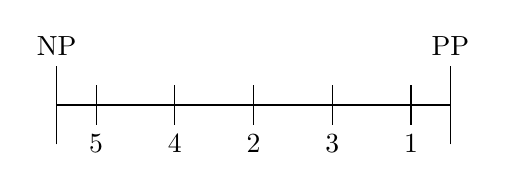
\begin{tikzpicture}
            \draw(0,0) -- (5,0);
            \draw (0,-0.5) -- (0,0.5);
            \node[anchor=south] at (0,0.5) {NP};
            \draw (5,-0.5) -- (5,0.5);
            \node[anchor=south] at (5,0.5) {PP};

            \node[anchor=north] at (0.5,-0.25) {5};
            \draw (0.5,-0.25) -- (0.5,0.25);

            \node[anchor=north] at (1.5,-0.25) {4};
            \draw (1.5,-0.25) -- (1.5,0.25);
            
            \node[anchor=north] at (2.5,-0.25) {2};
            \draw (2.5,-0.25) -- (2.5,0.25);
            
            \node[anchor=north] at (3.5,-0.25) {3};
            \draw (3.5,-0.25) -- (3.5,0.25);
            
            \node[anchor=north] at (4.5,-0.25) {1};
            \draw (4.5,-0.25) -- (4.5,0.25);
            
        \end{tikzpicture}
    \label{teehee}
    \end{center}
    \caption{A line drawing of the problem: \textit{If it were discovered that cell phones invariably and directly cause cancer, what should happen?} The numbers refer to scenarios outlined in Section~\ref{sec:linedrawing}.}
    \label{teehee}
\end{figure}

I propose this order, because I think that, in general, the more things are done voluntarily the better. Hence why the Positive Paradigm does not require government interference, and why 3) is placed above 2). In this case, where cell phones lead essentially directly to the deaths of their users, I do think that their use and use of any radio frequencies would have to be discontinued. There is, however, nuance in how quickly such a shift would occur, due to how much disruption it would cause.

\subsection{Flowchart Creation}
\label{sec:flowchartCreation}

The ethical scenarios and considerations would be different if radio frequencies only increased the risk of cancer, as opposed to directly causing it. For this scenario, we can use the flowchart approach. The flowchart is shown in Figure~\ref{theflowchart}.

\begin{figure}[h]
\begin{center}
    \includegraphics[width=7cm]{./flowchart.png}
    \caption{A flowchart for the question: \textit{If smartphones increase the risk of cancer, should they be sold?}}
    \label{theflowchart}
\end{center}
\end{figure}

In this flowchart, we take the position of the company looking to sell smartphones. This is, of course, an oversimplification of the problem. Essentially, those looking to sell their smartphones must ask several ethical questions, from obvious ones such as ``Is it legal?" to more difficult ones like ``Are the risks reasonable?" Some of these involve judgment calls that reasonable people can---and will---disagree on.

Both of the scenarios in this section were hypothetical, since there are not yet conclusive studies on this issue. The more pressing question is what to do right now, while we do not know the full effects.

\section{The Ethics if Cell-Phone-Cancer Research is Inconclusive}
This, of course, is the scenario we are currently in. The question is: \textit{Is it ethical to sell a product without full knowledge of the health risks it poses?} The surface-level answer is easy: of course its ethical, since we can never know everything about the health risks of every product.

The real world, however, is more complicated. The magnitude of the risk matters greatly. The proportion of studies that fail to demonstrate a link between smartphone radio frequencies and cancer certainly does not prove that there is no link. However, overall, the risk that there is a substantial increase in cancer risk from these devices would seem---to the best of our knowledge---to be relatively small, as years of research still cannot prove any kind of link with cancer. In general, as long as the risk is not substantial, I believe it is ethical to sell a product without knowing in full its potential for negative health effects. I think this applies in the current smartphone case. This is not to say that thorough research into the potential harms of the product is not necessary. More study in this area is important.

\section{Group Impacts: Responsibility and Injury}
In the issue at hand, it is important to recognize the impact smartphone-caused cancer will have. First, we will consider where responsibility lies for the oversight, and then the impact the oversight will have on the public.

\subsection{Responsibility}
The responsibility for this hypothetical oversight would be shared by many, and would be analogous to the responsibility of groups currently in charge of ensuruing the safety of radio frequency devices. These groups include engineers and scientists, regulatory boards, corporations, manufacturers, and consumers. We can rank these groups from most to least responsible.

The group most responsible is, of course, engineers and scientists. Engineers are the ones creating a product, and they have a duty to speak up when they believe the product they create is unsafe. Scientists researching the safety of products must report results without bias. Creating a product that is known to be harmful is never ethical. This is not to discount nuanced situations when there are certain \textit{risks} of harm that can be balanced and mitigated.

Next in responsibility are corporations and manufacturers. As the business entitees selling either parts for a product or the product itself, these groups must ensure they do not offer to people something they know is harmful. They are not as responsible as engineers because engineers should not have made a harmful product in the first place, but it is the corporations' and manufacturers' responsibility to ensure they do not sell a harmful product even if their engineers develop one.

Regulatory boards bear the next amount of responsibility, as they are a last stop between corporations selling potentially harmful products and the consumers. The regulatory boards, in an ideal world, would not have to exist because everyone above them would not create harmful products.

Lastly, consumers bear the least responsibility. Although consumers should look out for their safety, they have a right to expect that products legally on the market are safe to use.

\subsection{Consequences}
Among the groups above, which would be injured the most by a harmful ubiquitous product like a hypothetical cancer-causing smartphone.

Consumers are the obvious answer, since they have the least say in how their products function, but bear the brunt of any ill effects. Further, many consumers are not educated enough to know all the nuance of risk in a complicated device like a smartphone, so many will not have had enough knowledge to make an informed decision.

Engineers, corporations, and manufacturers would all receive about the same amount of injury. Aside from the physical effects that people working in these groups would also suffer, the entities themselves would only receive injury to reputation and monetary consequences, which is not comparable to the human suffering affecting the consumers.

Lastly, regulatory boards would, as entities, receive the least injury since there would not be any monetary consequences.




% An example of a floating figure using the graphicx package.
% Note that \label must occur AFTER (or within) \caption.
% For figures, \caption should occur after the \includegraphics.
% Note that IEEEtran v1.7 and later has special internal code that
% is designed to preserve the operation of \label within \caption
% even when the captionsoff option is in effect. However, because
% of issues like this, it may be the safest practice to put all your
% \label just after \caption rather than within \caption{}.
%
% Reminder: the "draftcls" or "draftclsnofoot", not "draft", class
% option should be used if it is desired that the figures are to be
% displayed while in draft mode.
%
%\begin{figure}[!t]
%\centering
%\includegraphics[width=2.5in]{myfigure}
% where an .eps filename suffix will be assumed under latex, 
% and a .pdf suffix will be assumed for pdflatex; or what has been declared
% via \DeclareGraphicsExtensions.
%\caption{Simulation results for the network.}
%\label{fig_sim}
%\end{figure}

% Note that the IEEE typically puts floats only at the top, even when this
% results in a large percentage of a column being occupied by floats.


% An example of a double column floating figure using two subfigures.
% (The subfig.sty package must be loaded for this to work.)
% The subfigure \label commands are set within each subfloat command,
% and the \label for the overall figure must come after \caption.
% \hfil is used as a separator to get equal spacing.
% Watch out that the combined width of all the subfigures on a 
% line do not exceed the text width or a line break will occur.
%
%\begin{figure*}[!t]
%\centering
%\subfloat[Case I]{\includegraphics[width=2.5in]{box}%
%\label{fig_first_case}}
%\hfil
%\subfloat[Case II]{\includegraphics[width=2.5in]{box}%
%\label{fig_second_case}}
%\caption{Simulation results for the network.}
%\label{fig_sim}
%\end{figure*}
%
% Note that often IEEE papers with subfigures do not employ subfigure
% captions (using the optional argument to \subfloat[]), but instead will
% reference/describe all of them (a), (b), etc., within the main caption.
% Be aware that for subfig.sty to generate the (a), (b), etc., subfigure
% labels, the optional argument to \subfloat must be present. If a
% subcaption is not desired, just leave its contents blank,
% e.g., \subfloat[].


% An example of a floating table. Note that, for IEEE style tables, the
% \caption command should come BEFORE the table and, given that table
% captions serve much like titles, are usually capitalized except for words
% such as a, an, and, as, at, but, by, for, in, nor, of, on, or, the, to
% and up, which are usually not capitalized unless they are the first or
% last word of the caption. Table text will default to \footnotesize as
% the IEEE normally uses this smaller font for tables.
% The \label must come after \caption as always.
%
%\begin{table}[!t]
%% increase table row spacing, adjust to taste
%\renewcommand{\arraystretch}{1.3}
% if using array.sty, it might be a good idea to tweak the value of
% \extrarowheight as needed to properly center the text within the cells
%\caption{An Example of a Table}
%\label{table_example}
%\centering
%% Some packages, such as MDW tools, offer better commands for making tables
%% than the plain LaTeX2e tabular which is used here.
%\begin{tabular}{|c||c|}
%\hline
%One & Two\\
%\hline
%Three & Four\\
%\hline
%\end{tabular}
%\end{table}


% Note that the IEEE does not put floats in the very first column
% - or typically anywhere on the first page for that matter. Also,
% in-text middle ("here") positioning is typically not used, but it
% is allowed and encouraged for Computer Society conferences (but
% not Computer Society journals). Most IEEE journals/conferences use
% top floats exclusively. 
% Note that, LaTeX2e, unlike IEEE journals/conferences, places
% footnotes above bottom floats. This can be corrected via the
% \fnbelowfloat command of the stfloats package.




\section{Conclusion}
In conclusion, much of the ethics of this issue come down to a risk assessment. Is there a risk associated with use of these devices? Yes, there is---at least until the radio-frequency-cancer link is scientifically disproven. Are there benefits that potentially outweigh those risks? Absolutely. Because there are both risks and benefits, and because the risks are not certain, it seems to be unnecessary to insist on a total ban on radio frequencies until we understand the cancer link better. Indeed, with our current understanding of the issues discussed in this paper, I believe the benefits of our use of radio frequencies greatly outweigh the small risks associated with our lack of understanding of the link between them and cancer. However, further study is important, as a definitive answer is necessary to truly assess the risks and benefits of these devices, especially considering their ubiquity.





% if have a single appendix:
%\appendix[Proof of the Zonklar Equations]
% or
%\appendix  % for no appendix heading
% do not use \section anymore after \appendix, only \section*
% is possibly needed

% use appendices with more than one appendix
% then use \section to start each appendix
% you must declare a \section before using any
% \subsection or using \label (\appendices by itself
% starts a section numbered zero.)
%


\appendices
% by themselves when using endfloat and the captionsoff option.
\ifCLASSOPTIONcaptionsoff
  \newpage
\fi



% trigger a \newpage just before the given reference
% number - used to balance the columns on the last page
% adjust value as needed - may need to be readjusted if
% the document is modified later
%\IEEEtriggeratref{8}
% The "triggered" command can be changed if desired:
%\IEEEtriggercmd{\enlargethispage{-5in}}

% references section

% can use a bibliography generated by BibTeX as a .bbl file
% BibTeX documentation can be easily obtained at:
% http://mirror.ctan.org/biblio/bibtex/contrib/doc/
% The IEEEtran BibTeX style support page is at:
% http://www.michaelshell.org/tex/ieeetran/bibtex/
%\bibliographystyle{IEEEtran}
% argument is your BibTeX string definitions and bibliography database(s)
%\bibliography{IEEEabrv,../bib/paper}
%
% <OR> manually copy in the resultant .bbl file
% set second argument of \begin to the number of references
% (used to reserve space for the reference number labels box)
\begin{thebibliography}{1}

\bibitem{cancersoc}
American Cancer Society. ``Radiofrequency (RF) Radiation." https://www.cancer.org/cancer/risk-prevention/radiation-exposure/radiofrequency-radiation.html, Oct. 28, 2022 (accessed Dec. 13, 2024).

\bibitem{fcc}
FCC. ``Wireless Devices and Health Concerns." https://www.fcc.gov/consumers/guides/wireless-devices-and-health-concerns, Nov. 4, 2020 (accessed Dec. 13, 2024).

\bibitem{itriplee}
IEEE. ``IEEE Standard for Safety Levels with Respect to Human Exposure to Electric, Magnetic, and Electromagnetic Fields, 0 Hz to 300 GHz," in IEEE Std C95.1-2019 (Revision of IEEE Std C95.1-2005/ Incorporates IEEE Std C95.1-2019/Cor 1-2019), 4 Oct. 2019.

\end{thebibliography}

\bigskip

\textbf{John Colton} is an Electrical Engineering student at the University of Mary in Bismarck, ND.

% You can push biographies down or up by placing
% a \vfill before or after them. The appropriate
% use of \vfill depends on what kind of text is
% on the last page and whether or not the columns
% are being equalized.

%\vfill

% Can be used to pull up biographies so that the bottom of the last one
% is flush with the other column.
%\enlargethispage{-5in}



% that's all folks
\end{document}